\documentclass{beamer}

\makeatletter
\def\normaljustify{%
  \let\\\@centercr\rightskip\z@skip \leftskip\z@skip%
  \parfillskip=0pt plus 1fil}
\makeatother
\usetheme{Singapore}

\title{Visual Analytics on Human Body Movement Data }
\subtitle{Applied on Healthcare}
\author{Oky Purwantiningsih}
\institute{IT4BI Master Thesis}
\date{\today}


\begin{document}
\begin{frame}
\titlepage
\end{frame}

\begin{frame}
\label{contents}
\frametitle{Outline}
\tableofcontents
\end{frame}

%=================================
\section{Introduction}
%\subsection{Motivation}
\begin{frame}
\frametitle{Motivation}
\begin{columns}
\column{0.5\textwidth}
\centering
\begin{figure}
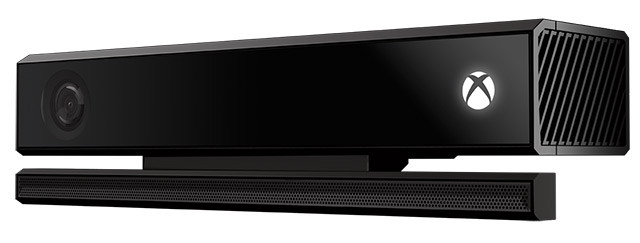
\includegraphics[width=3.5cm,height=1.7cm]{images/kinect.jpg}
\caption{Kinect}
\end{figure}
\begin{figure}
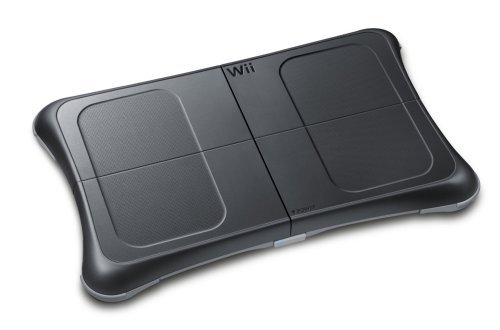
\includegraphics[width=3.5cm,height=1.7cm]{images/wii_balance_board.jpg}
\caption{Wii Balance Board}
\end{figure}

\column{0.5\textwidth}
\centering
\begin{figure}
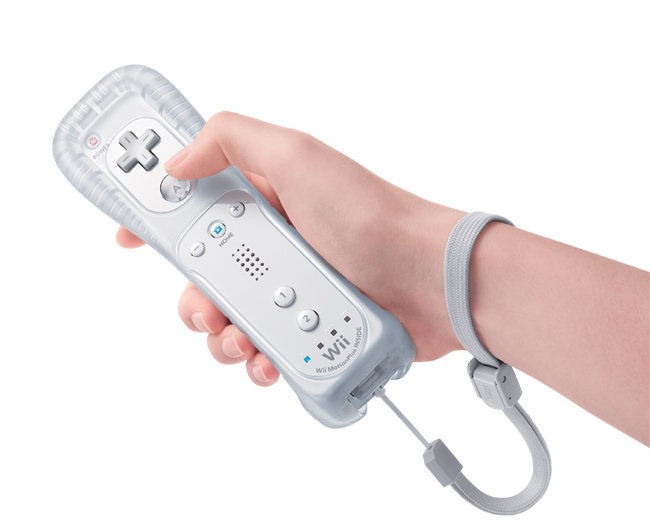
\includegraphics[width=3.5cm,height=1.7cm]{images/wii_remote.jpg}
\caption{Wii Remote}
\end{figure}
\begin{figure}
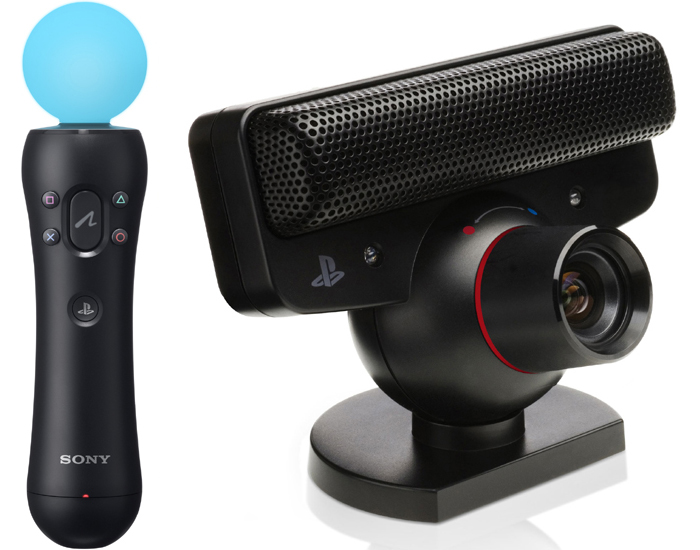
\includegraphics[width=3.5cm,height=1.7cm]{images/play_station_move.jpg}
\caption{Play Station Move}
\end{figure}

\end{columns}
Motion Sensing input devices enable players to control and interact with the game console through body movement.
\end{frame}

\begin{frame}
\frametitle{Motivation}
\centering
\begin{figure}
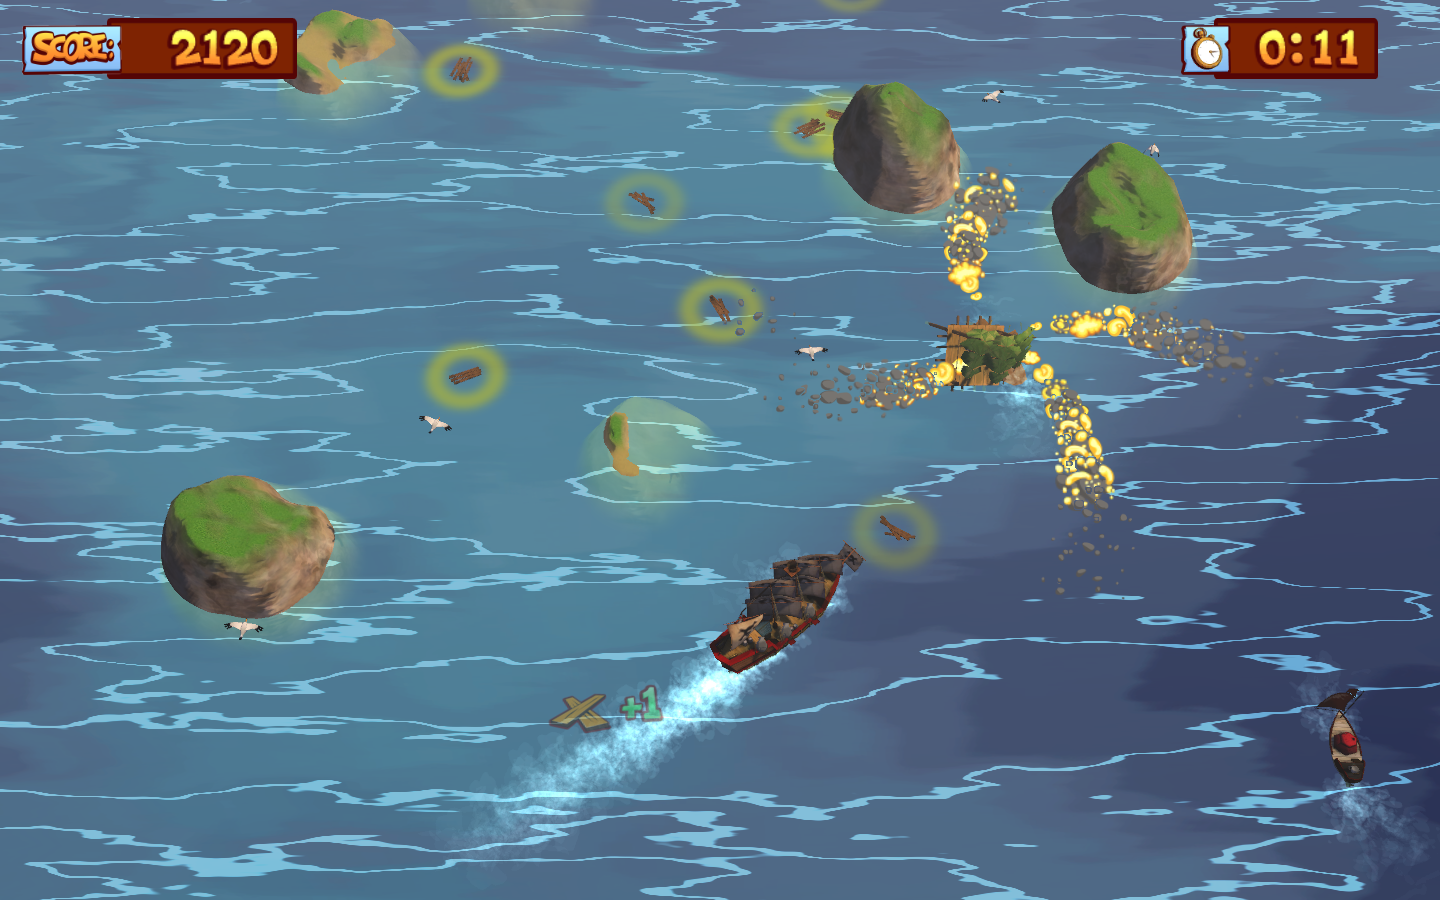
\includegraphics[scale=0.16]{images/hp_game.png}
\caption{Hammer and Planks Interface}
\end{figure}

\normaljustify
\begin{itemize}
\item Hammer and Planks is a serious game designed to train the equilibrium of patient with balance disorders (ie. Hemiplegic people).\\
\item Players are required to move their body parts to the right, left, backward, and forward as part of the rehabilitation
\item Game missions: collect bonuses, kill enemies, avoid obstacles
\end{itemize}

\end{frame}

\begin{frame}
\frametitle{Motivation}
With current visualization, the information

Available:
\begin{itemize}
\item Average degree of body movement over x axis
\item Average degree of body movement over y axis
\end{itemize}

Not Available:
\begin{itemize}
\item How often the player move to right or left?
\item To which type of events (collecting bonuses, killing enemies) the movement is related?
\item Evolution of player's movement
\end{itemize}

\end{frame}

%\subsection{Methodology}
\begin{frame}
\frametitle{Methodology}
\centering
\begin{figure}
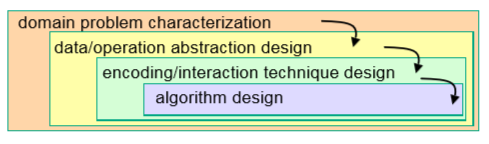
\includegraphics[scale=0.7]{images/munzner_model.png}
\caption{Munzner's Visualization Design Model}
\end{figure}

\normaljustify
\begin{itemize}
\item What kind of information needed by health professionals from the visualization (List of Tasks)
\item Define data structure to support the tasks
\item Define visualization and interaction technique
\end{itemize}
\end{frame}

%=================================
\section{Domain Problem Characterization}
%\subsection{Hammer and Planks Game Dynamic}
\begin{frame}
\frametitle{Hammer and Planks Game Dynamic}
\begin{columns}
\column{0.5\textwidth}
\centering
\begin{figure}
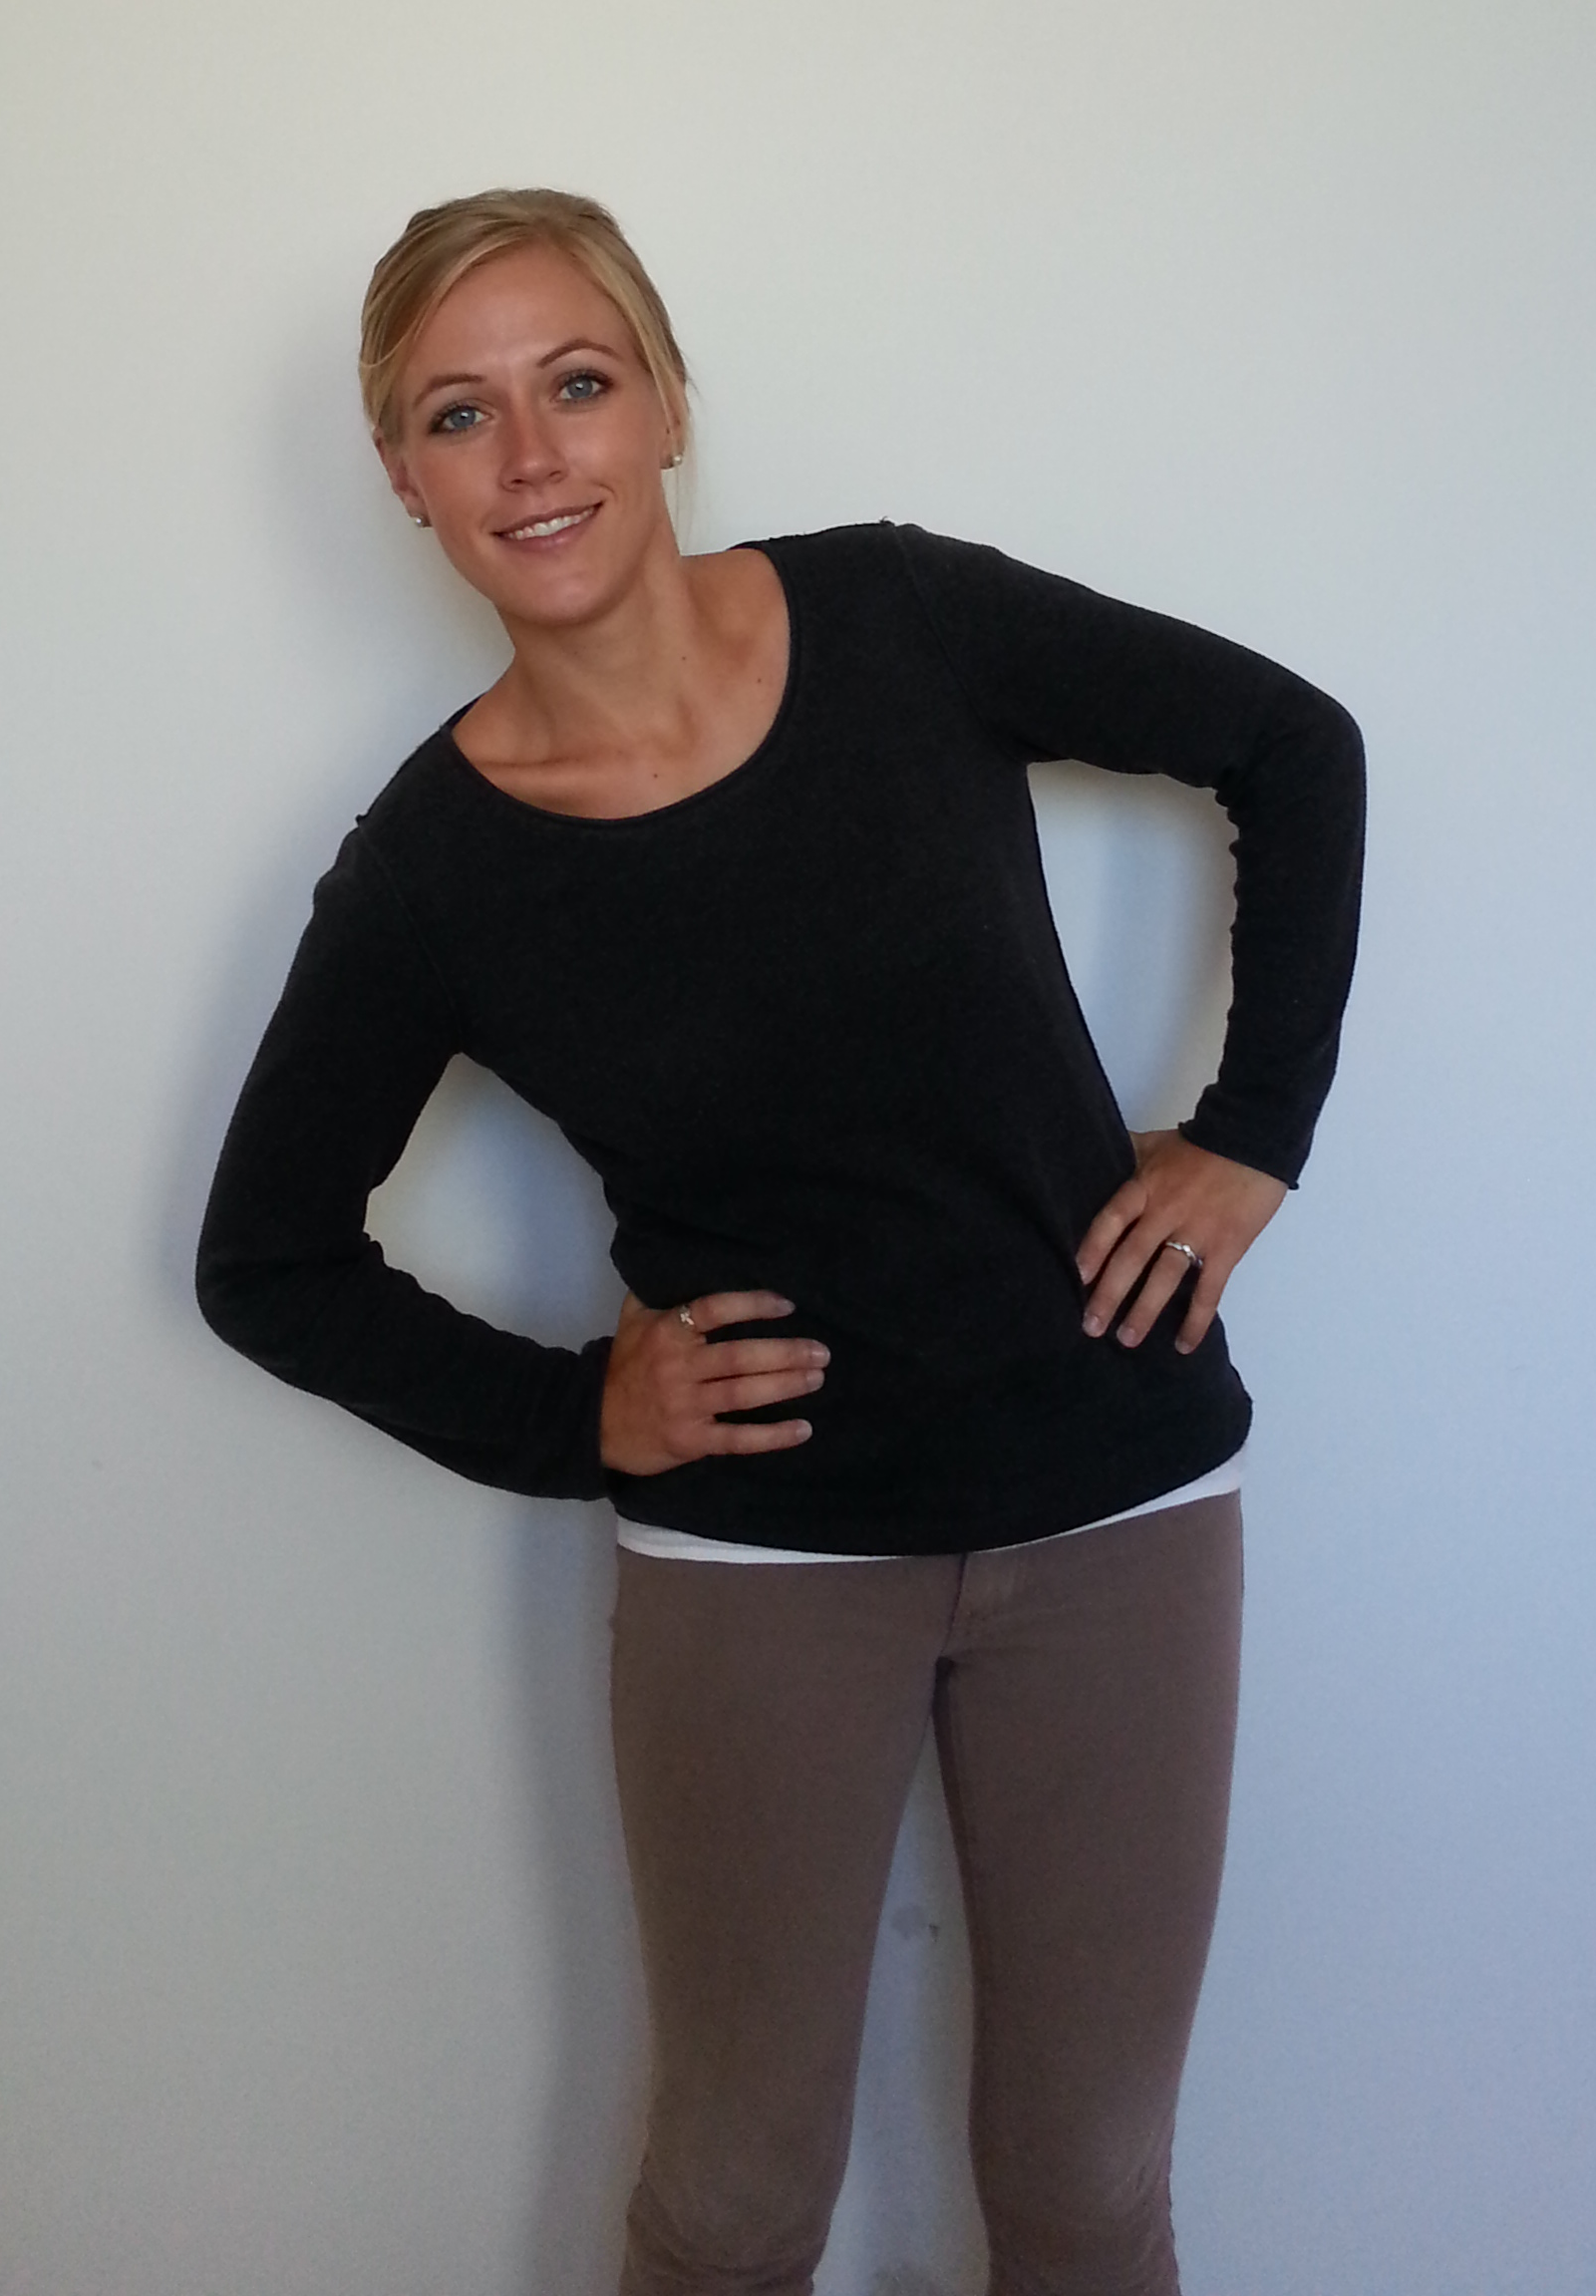
\includegraphics[scale=0.06]{images/mia_bodytilt.png}
\caption{BodyTilt}
\end{figure}

\column{0.5\textwidth}
\centering
\begin{figure}
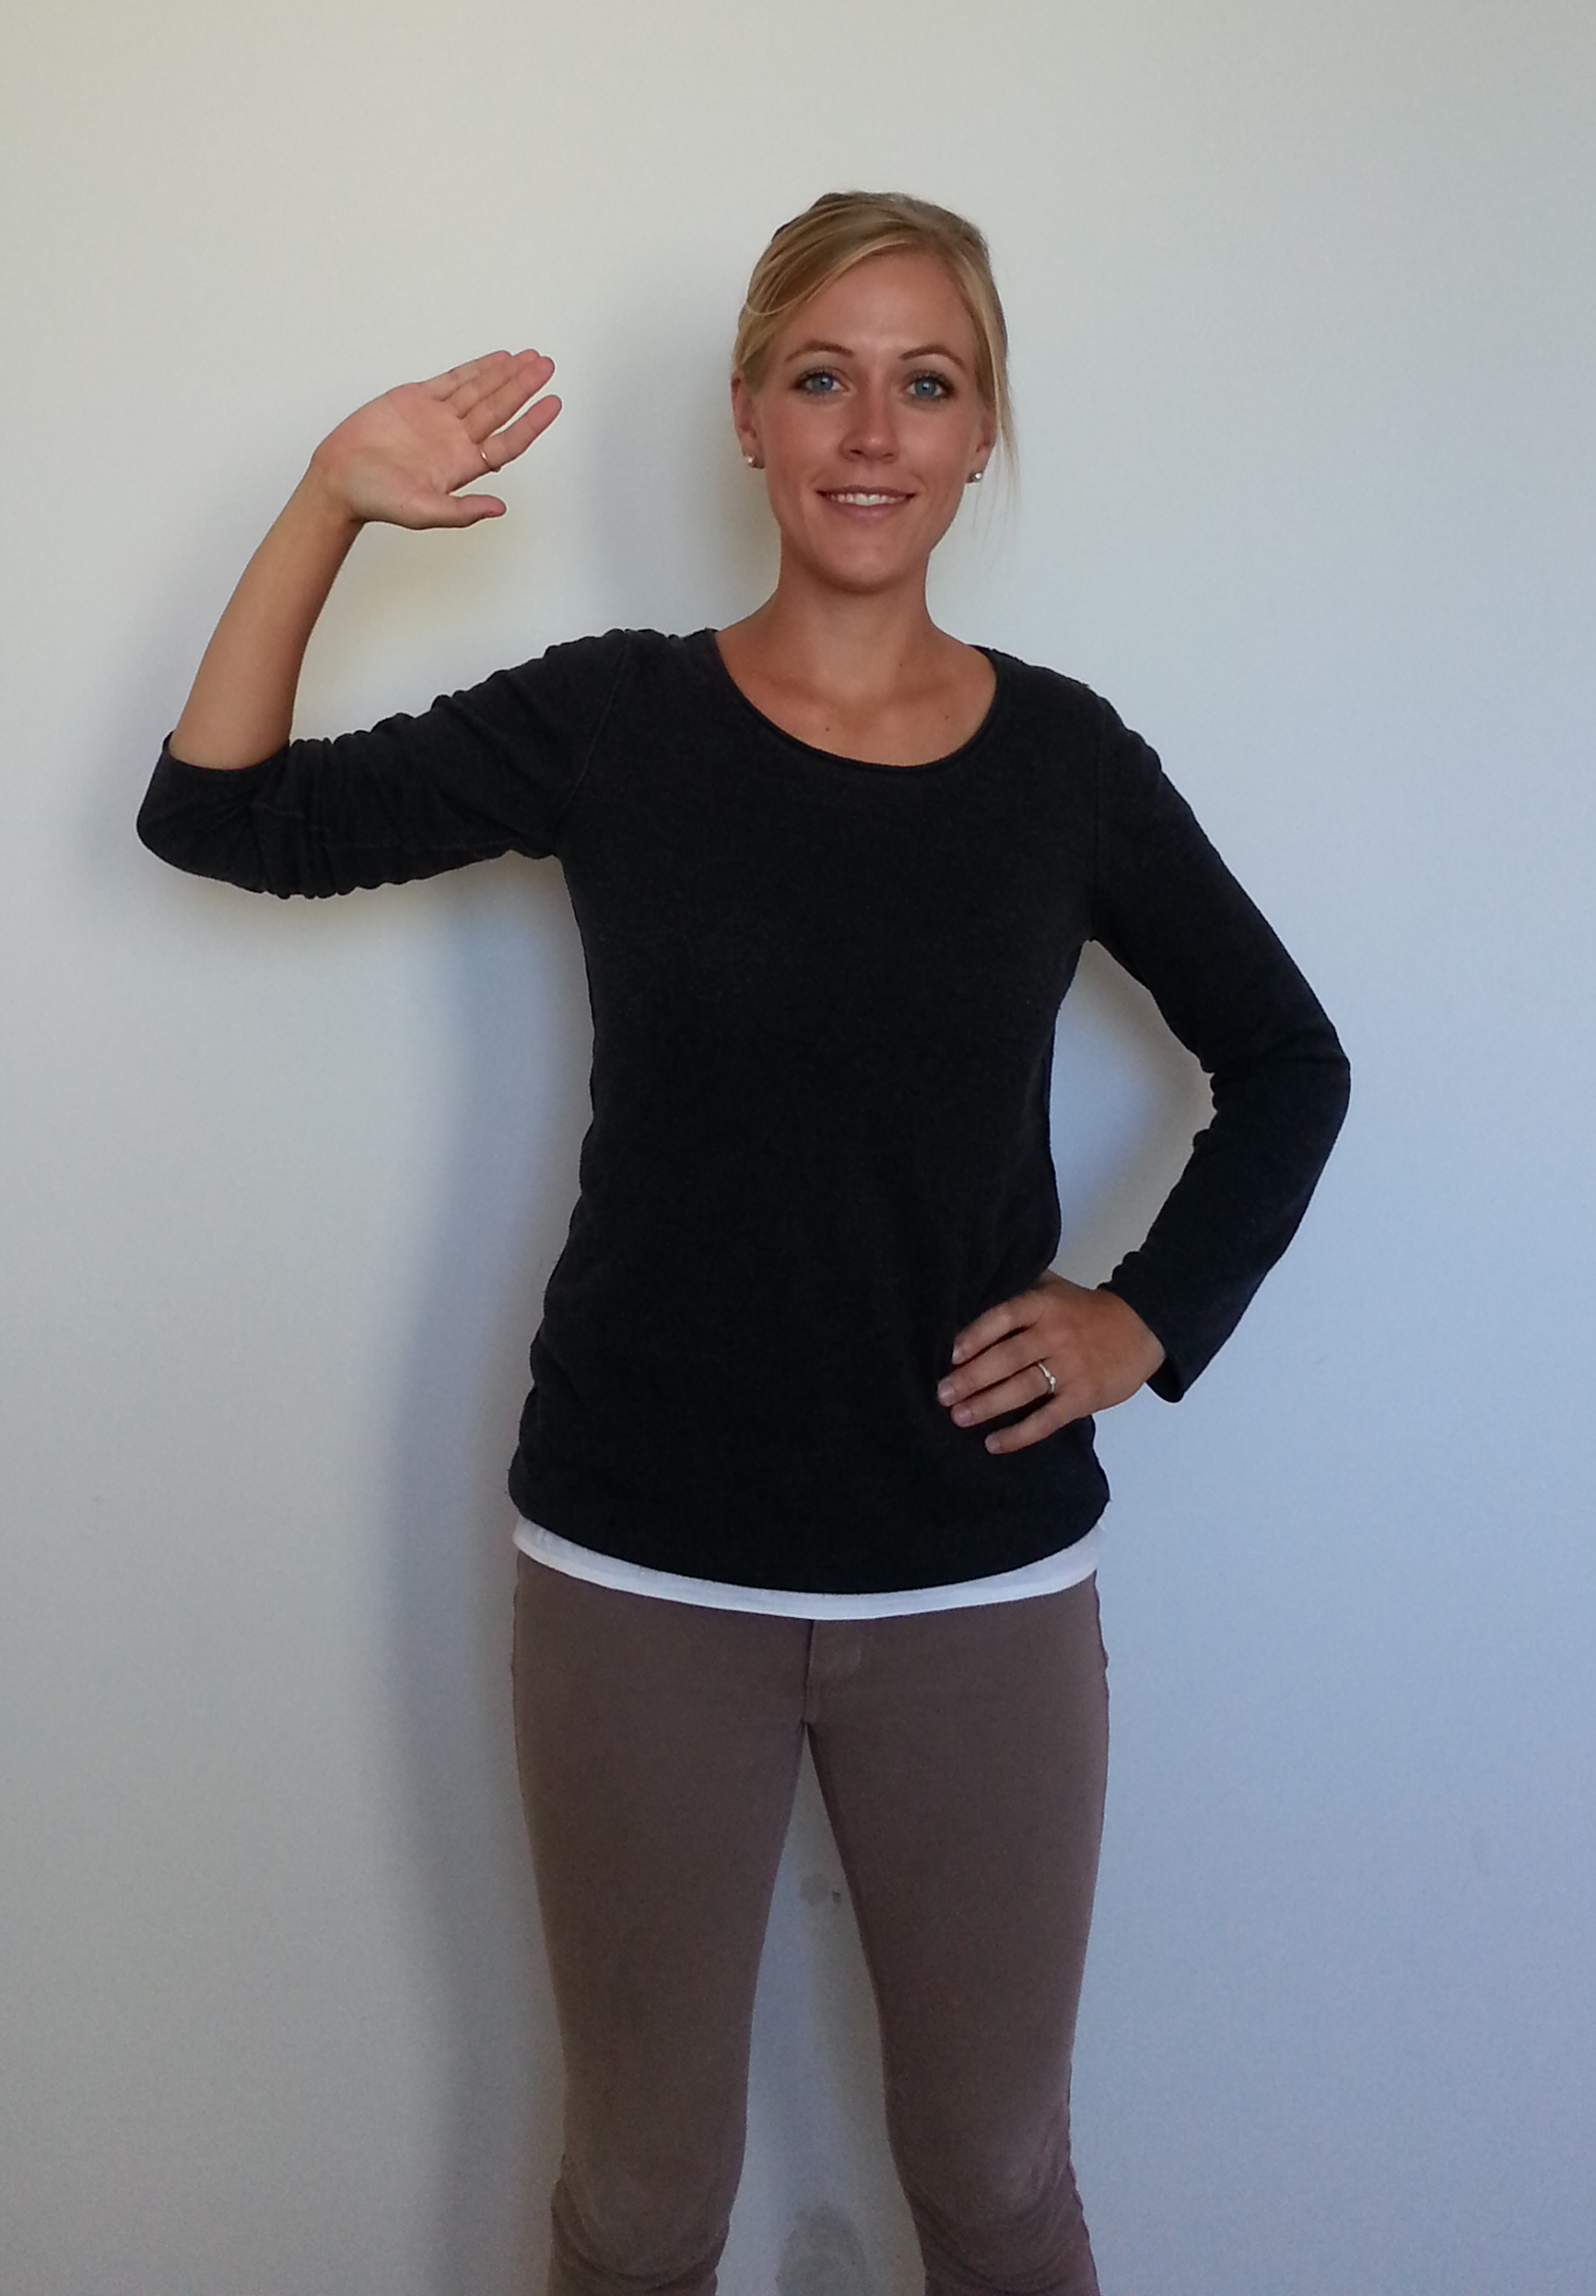
\includegraphics[scale=0.06]{images/mia_handpoint.png}
\caption{HandPoint}
\end{figure}

\end{columns}
\begin{itemize}
\item Healthcare professional can adjust game difficulty by setting the number of objects, area where objects can appear, activity duration and repetition
\item Movement Setting: BodyTilt, HandPoint, ShoulderCGE
\item Game Direction: Vertical, Horizontal, Both
\end{itemize}
\end{frame}

%\subsection{Target User Question}
\begin{frame}
\frametitle{Target User Question}
(Q1) For a given session, to which direction (right/left) the player moved more?\\ 
(Q2) For a given session, how does the player perform based on the number of objects collected, avoided, or killed with respect to the area of the movement?\\
(Q3) For a given session, how does the player perform based on the number of objects collected, avoided, or killed with respect to the area of movement and the speed in which the game is played?\\ 
(Q4) For a given patient, has he/she has improved in the game overtime?\\ 
(Q5) For a given patient, has he/she has improved in a certain area overtime?


\end{frame}

%\subsection{Visualization Requirements}
\begin{frame}
\frametitle{Visualization Requirements}
Tasks related to a session of a particular player:\\
(T1.1) visualize and be able to compare the number of events within the same or among different event type at a given x area (Q1)(Q2). \\
(T1.2) visualize and be able to compare the number of events and its screen speed of the same or among different event type at a given x area (Q1)(Q2)(Q3). \\
(T1.3) select and visualize the number of events for a certain object at a given x area (Q1)(Q2). \\
(T1.4) select and visualize the number of events and its screen speed for a certain object at a given x area (Q1)(Q2)(Q3). 
\end{frame}

\begin{frame}
\frametitle{Visualization Requirements}
Tasks related to the summary of all sessions of a player:\\
(T2.1) visualize, navigate and be able to compare the evolution of number of events throughout all sessions within a certain x area.(Q4)(Q5). \\
(T2.2) select and visualize the number of events of a certain event type in a certain x area throughout all sessions (Q4)(Q5).\\ 
(T2.3) visualize, navigate and be able to compare the distribution of a certain number of events over x area among all sessions(Q4)(Q5). \\
(T2.4) select and visualize the distribution of certain number of events over x area for a certain event type throughout all sessions (Q4)(Q5). \\
(T2.5) extract and visualize similar pattern of number of events evolution throughout all sessions over a certain x area (Q4)(Q5).
\end{frame}
%=================================
\section{Related Works}
%\subsection{Visualization of Serious Game Result}
\begin{frame}
\frametitle{Visualization of Serious Game Result}
\begin{figure}
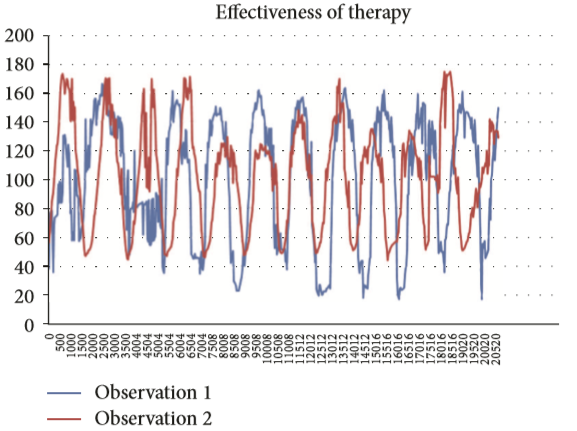
\includegraphics[scale=0.5]{images/rahman_viz.png}
\caption{Line Chart depicting degree of forearm movement over time}
\end{figure}
\end{frame}


%\subsection{Visualization of Time Series Data}

\begin{frame}
\frametitle{Visualization of Time Series Data}
\begin{figure}
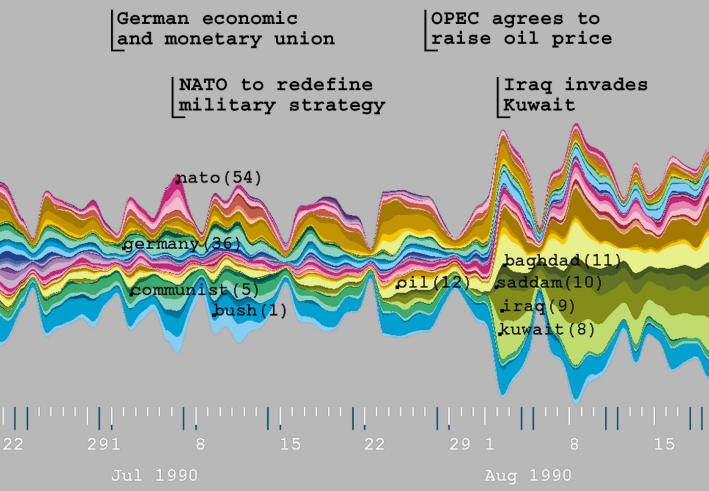
\includegraphics[scale=0.5]{images/havre_themeriver.png}
\caption{Theme River}
\end{figure}
\end{frame}

%\subsection{Visualization of Movement Data}

\begin{frame}
\frametitle{Visualization of Movement Data}
\begin{figure}
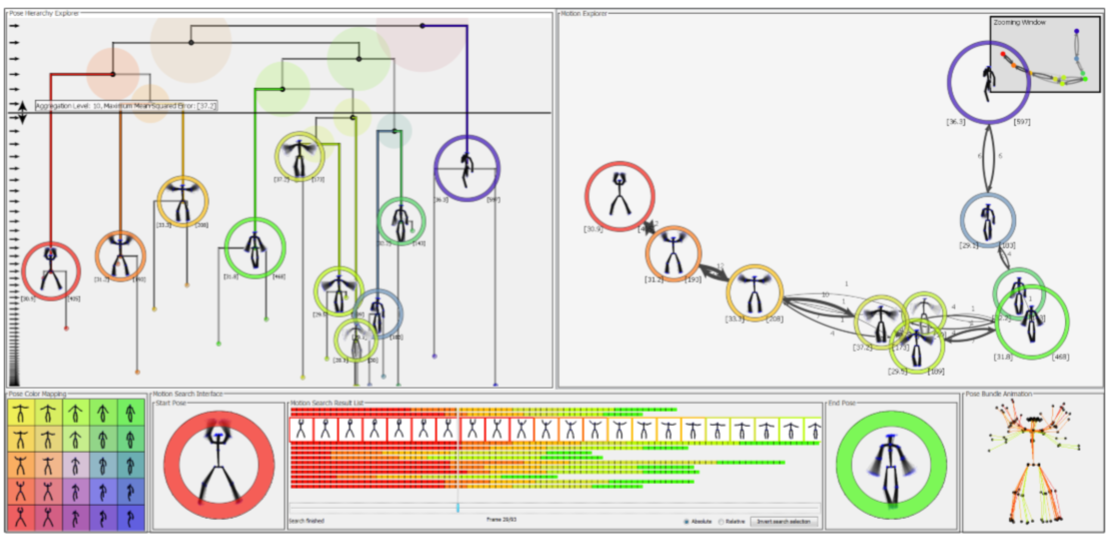
\includegraphics[scale=0.4]{images/bernard_motionexplorer.png}
\caption{Motion Explorer}
\end{figure}
\end{frame}

%=================================
\section{Data Abstraction}
%\subsection{Game Events Structure}
\begin{frame}
\frametitle{Game Events Structure}
\begin{itemize}
\item Event Category: Positive, Neutral, Negative
\begin{table}[h]
\begin{center}
    \begin{tabular}{| l | l | l | l |}
    \hline
    Events & Bonus & Obstacle & Enemy \\ \hline
    Positive & catch & - & kill,hit\\ \hline
    Neutral & miss & dodge & miss\\ \hline
    Negative & - & collision & hurt, collision\\
    \hline
    \end{tabular}
    \label{tblEventType}
\end{center}
\end{table}
\item Screen Speed: distance between apparition location and event location divided by duration between apparition time and event time
$$ \upsilon_{scr} = \frac{\theta_{evt}-\theta_{apr}}{\textit{t}_{evt}-\textit{t}_{apr}} $$
\end{itemize}
\end{frame}

%\subsection{Clustering}
\begin{frame}
\frametitle{Clustering - Distance Calculation}
\begin{itemize}
\item To see common evolution of different section of x-area, consecutive sections with similar movement distribution are clustered together
\item Let S be a gameplay data set of $n_{ses}$ sessions. 
\item S is an ordered list of sections $s_i, 0 \le i < n_{sec}$. Each section contains events occurred on an x-axis unit among all sessions. 
\item A section $s_i$ is a sequence of triplets $s_i\lbrack j \rbrack, 0 \le j < n_{ses}$. Each triplet represents data set of a certain game session of a particular section $s_i$. 
\item The triplet consists of the number of negative, neutral and positive events. 
\item The profile of each section can be represented by a matrix of $n_{ses}$ x 3 dimensions.
\end{itemize}
\[
\textit{s}_1 = \begin{bmatrix}
  10 & 20 & 6\\
  20 & 5 & 18
\end{bmatrix}
\textit{s}_2 = \begin{bmatrix}
  20 & 40 & 10\\ 
  40 & 10 & 30
\end{bmatrix}
\textit{s}_3 = \begin{bmatrix}
  10 & 20 & 5\\
  16 & 4 & 12 
\end{bmatrix}
\]
\end{frame}
\begin{frame}
\frametitle{Clustering - Distance Calculation}
\begin{itemize}
\item Similarity between two sections is quantified with distance function (distance=0:similar; distance=1: different)
\item Two types of distance: 
\begin{itemize}
\item How different both sections in term of event types proportion within each section ( $s_2$ is similar to $s_3$)
\item How different both sections in term of the evolution of each event type throughout the sessions ( $s_1$ is similar to $s_2$)
\end{itemize}
\[
\textit{s}_1 = \begin{bmatrix}
  10 & 20 & 6\\
  20 & 5 & 18
\end{bmatrix}
\textit{s}_2 = \begin{bmatrix}
  20 & 40 & 10\\ 
  40 & 10 & 30
\end{bmatrix}
\textit{s}_3 = \begin{bmatrix}
  10 & 20 & 5\\
  16 & 4 & 12 
\end{bmatrix}
\]
\item For each pair of consecutive sequences ($\textit{s}_1$,$\textit{s}_2$) of \textit{S}, distance is weighted sum of two distance types, represented as $\textit{f}(\textit{s}_1,\textit{s}_2)$ and $\textit{g}(\textit{s}_1,\textit{s}_2)$.

$$d(\textit{s}_1,\textit{s}_2) = \alpha\textit{f}(\textit{s}_1,\textit{s}_2) + (1 - \alpha)\textit{g}(\textit{s}_1,\textit{s}_2)$$
\end{itemize}


\end{frame}
\begin{frame}
\frametitle{Clustering - Distance Calculation}
\begin{itemize}


\item $f(\textit{s}_1,\textit{s}_2)$ is a normalized euclidean distance of two triplets.
\item Distance is the average euclidean distance of each triplets pair. 
$$f(\textit{s}_1,\textit{s}_2) = \frac{\displaystyle\sum_{i=0}^{i < \lvert\textit{s}_1\lvert} \textit{N}ED(\textit{s}_1\lbrack i \rbrack,\textit{s}_2\lbrack i \rbrack)}{ \lvert\textit{s}_1\lvert}$$
\item Distance is normalized by dividing it with maximum distance $\sqrt{3}$.
$$ \textit{N}ED(\textit{s}_1\lbrack i \rbrack,\textit{s}_2\lbrack i \rbrack) = \frac{\sqrt{\displaystyle\sum_{j \in \{0,1,2\}}(\textit{s}_1'\lbrack i \rbrack\lbrack j \rbrack - \textit{s}_2'\lbrack i \rbrack\lbrack j \rbrack)^2}}{\sqrt{3}}$$
\item $\textit{s}_1'$ and $\textit{s}_2'$ is normalized value of $\textit{s}_1$ and $\textit{s}_2$ (divided by max value of each session in each section)

\end{itemize}
\end{frame}

\begin{frame}
\frametitle{Clustering - Distance Calculation}
\[
\textit{s}_1 = \begin{bmatrix}
  10 & 20 & 6\\
  20 & 5 & 18
\end{bmatrix}
\textit{s}_2 = \begin{bmatrix}
  20 & 40 & 10\\ 
  40 & 10 & 30
\end{bmatrix}
\textit{s}_3 = \begin{bmatrix}
  10 & 20 & 5\\
  16 & 4 & 12 
\end{bmatrix}
\]

\[
s_1' = \begin{bmatrix}
  \frac{1}{2} & 1 & \frac{6}{20}\\ 
  1 & \frac{1}{4} & \frac{18}{20}
\end{bmatrix}
s_2' = \begin{bmatrix}
  \frac{1}{2} & 1 & \frac{1}{4}\\
  1 & \frac{1}{4} & \frac{3}{4} 
\end{bmatrix}
s_3' = \begin{bmatrix}
  \frac{1}{2} & 1 & \frac{1}{4}\\
  1 & \frac{1}{4} & \frac{3}{4} 
\end{bmatrix}
\]
\end{frame}
\begin{frame}
\frametitle{Clustering - Distance Calculation}
\begin{itemize}
\item $\textit{g}(\textit{s}_1,\textit{s}_2)$ is based on a normalized euclidean distance between the same event type \textit{j} from different section. 
\item The overall distance of both sections is the average euclidean distance of each event type pair. 
$$\textit{g}(\textit{s}_1,\textit{s}_2) = \frac{\textit{g}_0(\textit{s}_1,\textit{s}_2) + \textit{g}_1(\textit{s}_1,\textit{s}_2) + \textit{g}_2(\textit{s}_1,\textit{s}_2)}{3}$$
\item For each event type distance, there are three different distance value defined:
\begin{itemize}
\item if there are no events in both event type pairs, the distance is 0 
\item if there is at least one event in one section and there are no events in the other section, the distance is 1
\item if both event type pairs has any events then the euclidean distance is calculated
\end{itemize}

\end{itemize}
\end{frame}
\begin{frame}
\frametitle{Clustering - Distance Calculation}
for $j  \in \{0,1,2\}$,
\[g_j(\textit{s}_1,\textit{s}_2) = \left\{
  \begin{array}{ll}
    0 & \text{ if } \textit{s}_k\lbrack i \rbrack\lbrack j \rbrack=0 \text{ for each } 0 \leqslant j < |\textit{s}_k|\text{ and } \textit{k} \in \{1,2\}\\
    1 & \text{ if } \textit{s}_k\lbrack i \rbrack\lbrack j \rbrack=0 \text{ for each } 0 \leqslant j < |\textit{s}_k| \text{ and } \exists \textit{s}_p\lbrack i \rbrack\lbrack j \rbrack \neq 0,\\
      & k,p \in \{1,2\} \text{, } k \neq p\\
      & \\
	\multicolumn{2}{l}{\frac{\sqrt{\displaystyle\sum_{i=0}^{\lvert\textit{s}_1\lvert} (\textit{s}_1''\lbrack i \rbrack\lbrack j \rbrack - \textit{s}_2''\lbrack i \rbrack\lbrack j \rbrack)^2}}{\sqrt{\lvert\textit{s}_1\rvert}} \text{ otherwise}} 
  \end{array}
\right.
\]
\begin{itemize}
\item $s_1''$ and $s_2''$ represent normalized value of $s_1$ and $s_2$ (divided by max value of each event type in each section)

\end{itemize}
\end{frame}

\begin{frame}
\frametitle{Distance Calculation}
\[
\textit{s}_1 = \begin{bmatrix}
  10 & 20 & 6\\
  20 & 5 & 18
\end{bmatrix}
\textit{s}_2 = \begin{bmatrix}
  20 & 40 & 10\\ 
  40 & 10 & 30
\end{bmatrix}
\textit{s}_3 = \begin{bmatrix}
  10 & 20 & 5\\
  16 & 4 & 12 
\end{bmatrix}
\]

\[
s_1'' = \begin{bmatrix}
  \frac{1}{2} & 1 & \frac{1}{3}\\ 
  1 & \frac{1}{4} & 1
\end{bmatrix}
s_2'' = \begin{bmatrix}
  \frac{1}{2} & 1 & \frac{1}{3}\\ 
  1 & \frac{1}{4} & 1
\end{bmatrix}
s_3'' = \begin{bmatrix}
  \frac{5}{8} & 1 & \frac{5}{12}\\
  1 & \frac{1}{5} & 1 
\end{bmatrix}
\]
\end{frame}

\begin{frame}
\frametitle{Clustering Algorithm}
\begin{enumerate}
\item Divide data set into sections the size of x-axis unit
\item Calculate distance between two consecutive sections
\item Cluster sections with distance below threshold. This results in a new set of sections
\item Recalculate distance and cluster
\item Repeat the process until there is no sections with distance below the threshold
\end{enumerate}
\end{frame}

%=================================
\section{Visual Mappings and Interactive Functionality}
%\subsection{Session Visualization}
\begin{frame}
\frametitle{Session Visualization - Stacked Graph (T1.1)}
\begin{figure}
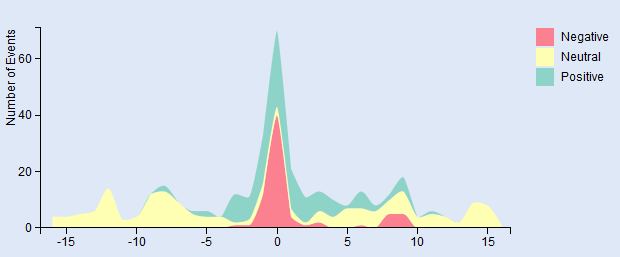
\includegraphics[scale=0.7]{images/stackedgraph_linear.png}
\caption{Stacked Graph depicting number of events over x axis}
\end{figure}
\end{frame}

\begin{frame}
\frametitle{Session Visualization - Stacked Graph Layout}
\begin{columns}
\column{0.5\textwidth}
\centering
\begin{figure}
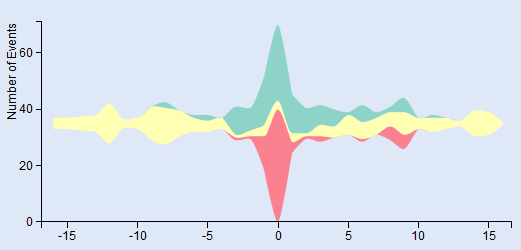
\includegraphics[width=5cm,height=2.4cm]{images/stackedgraph_silhouette.png}
\caption{Silhouette}
\end{figure}
\begin{figure}
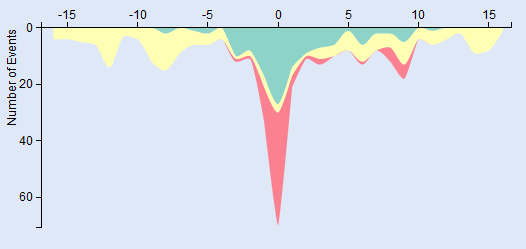
\includegraphics[width=5cm,height=2.4cm]{images/stackedgraph_positive.png}
\caption{Positive}
\end{figure}

\column{0.5\textwidth}
\centering
\begin{figure}
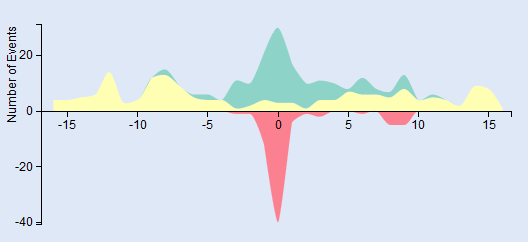
\includegraphics[width=5cm,height=2.4cm]{images/stackedgraph_neutral_neg.png}
\caption{Neutral-Negative}
\end{figure}
\begin{figure}
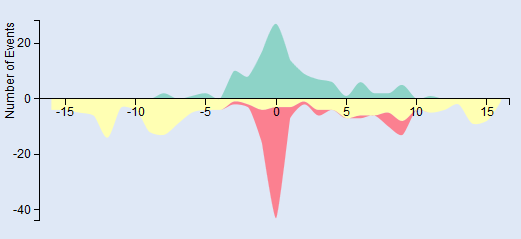
\includegraphics[width=5cm,height=2.4cm]{images/stackedgraph_positive_neutral.png}
\caption{Positive-Neutral}
\end{figure}

\end{columns}
\end{frame}

\begin{frame}
\frametitle{Session Visualization - Heatmap (T1.2)}
\begin{figure}
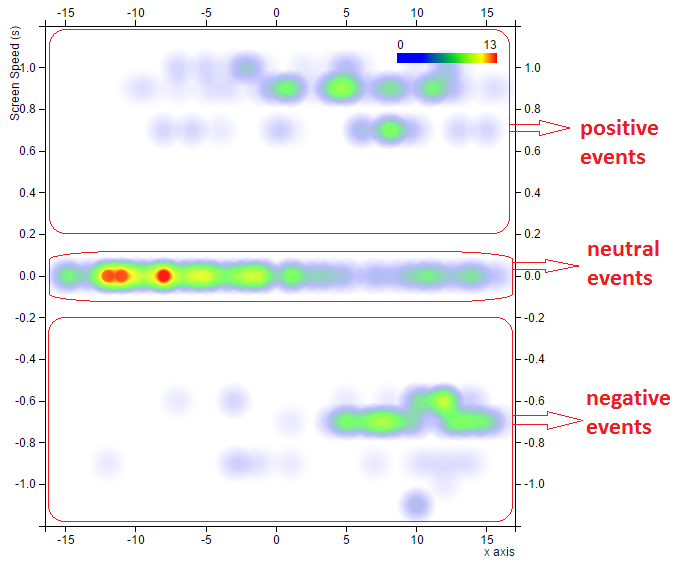
\includegraphics[scale=0.4]{images/heatmap3.png}
\caption{Heatmap depicting number of events and screen speed over x axis}
\end{figure}
\end{frame}

%\subsection{Summary Visualization}
\begin{frame}
\frametitle{Summary Visualization by range of x-area (T2.1)}
\begin{figure}
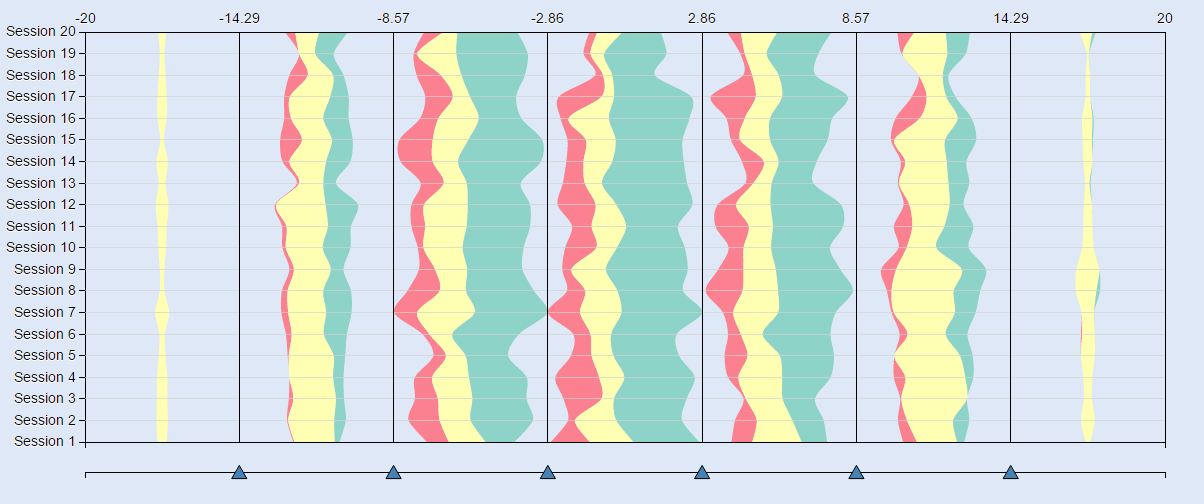
\includegraphics[scale=0.35]{images/summary_type1.png}
\caption{Summary Visualization by range of x-area: each section has the same x-range}
\end{figure}
\end{frame}
\begin{frame}
\frametitle{Summary Visualization by number of events (T2.3)}
\begin{figure}
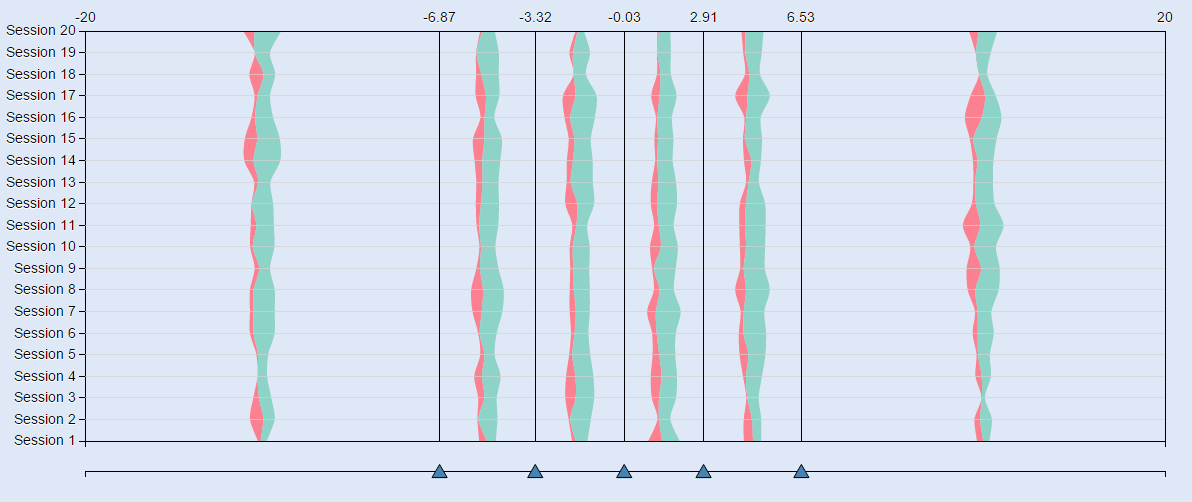
\includegraphics[scale=0.35]{images/summary_type2.png}
\caption{Summary Visualization by number of events: each section has the same number of positive and negative events}
\end{figure}
\end{frame}
\begin{frame}
\frametitle{Summary Visualization by clustering (T2.5)}
\begin{figure}
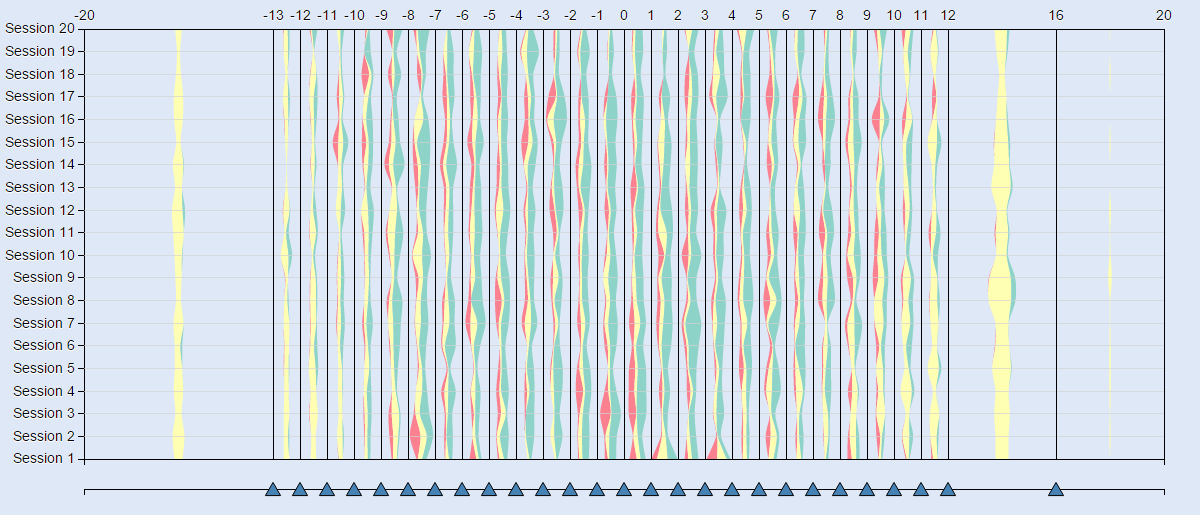
\includegraphics[scale=0.35]{images/summary_clustered.png}
\caption{Summary Visualization by clustering: each section has the similar movement pattern}
\end{figure}
\end{frame}
\begin{frame}
\frametitle{Summary Visualization - Interaction Technique(T2.2,T2.4)}
\begin{figure}
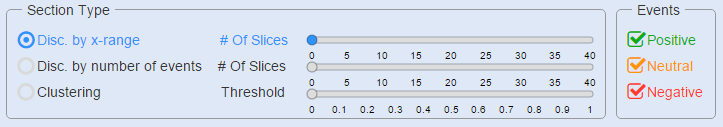
\includegraphics[scale=0.6]{images/interaction_bar.png}
\caption{Interaction bar allows user to choose which event type to show and change input using sliders}
\end{figure}
\end{frame}

\begin{frame}
\frametitle{Summary Visualization - Interaction Technique}
\begin{figure}
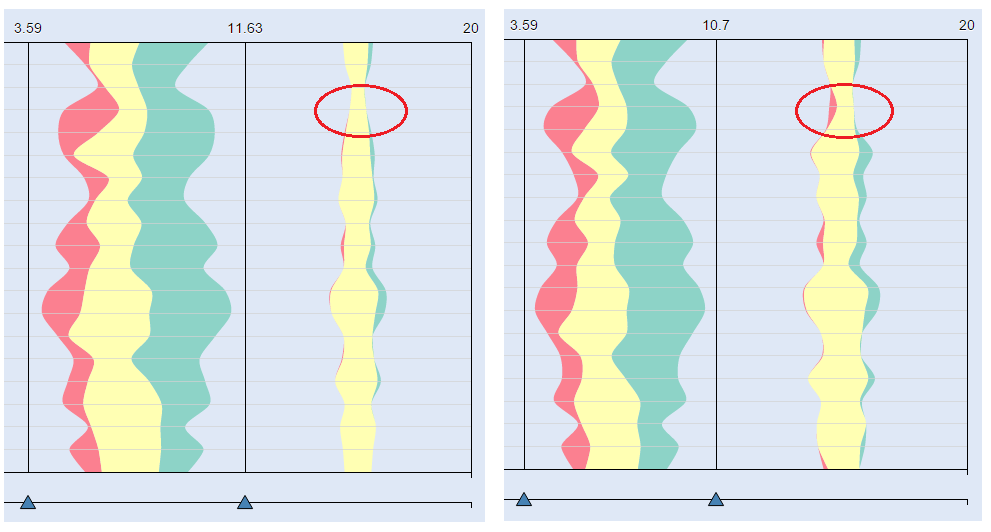
\includegraphics[scale=0.4]{images/line_dragging.png}
\caption{By dragging section line or triangle symbol, user can highlight movement pattern }
\end{figure}
\end{frame}
%\subsection{General Interface}
\begin{frame}
\frametitle{General Interface}
\begin{figure}
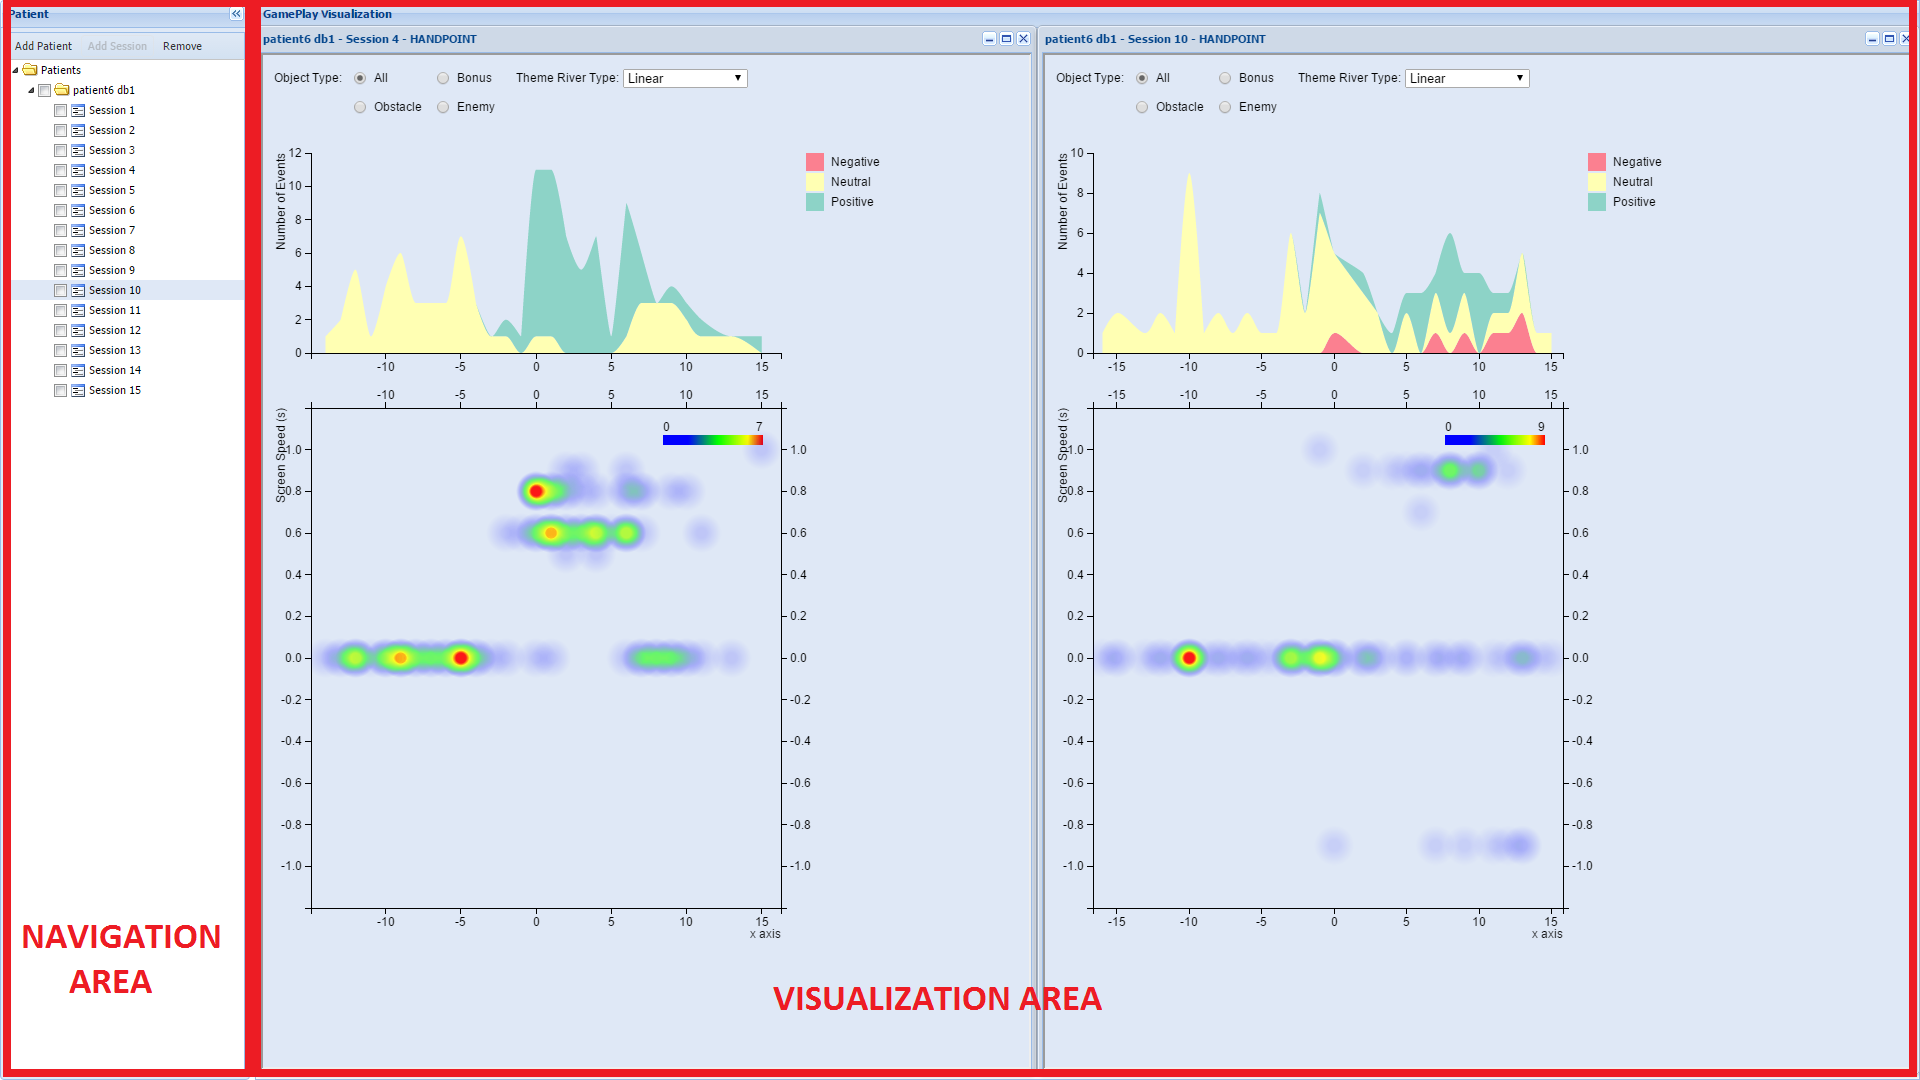
\includegraphics[scale=0.2]{images/interface_app_compare.png}
\caption{Interface is divided into two areas: navigation area and visualization area}
\end{figure}
\end{frame}

%=================================
\section{Case Study and Demo}
\begin{frame}
\frametitle{Case Study and Demo}
\begin{itemize}
\item Data set is acquired from NaturalPad
\item Data set is of game played by patient with pathology(type of pathology unknown)
\item Case study using HandPoint exercise, consists of 6 sessions
\end{itemize}

\end{frame}


%=================================
\section{Conclusion}
\begin{frame}
\frametitle{Conclusion}
\begin{itemize}
\item The proposed visualizations are able to provide information on movement direction, movement and its related events, movement evolution
\item Case study shows the effectiveness of the interface in achieving the tasks defined
\item Future Works:
\begin{itemize}
\item Improve clustering using different distance measure
\item Study on pathology and its movement to propose game setting based on pathology and its severity
\item Visualize log data related to skeleton movement
\end{itemize}
\end{itemize}
\end{frame}

\end{document}